% -*-latex-*-
\documentclass[pdftex,12pt,dvipsnames]{beamer}
\usepackage{etex,pictex,color}
\usepackage{graphicx}
\setbeamercovered{transparent}
\setbeamertemplate{footline}[frame number]
\begin{document}
\title{On: Paleolithic to Bronze Age Siberians Reveal Connections with
  First Americans and across Eurasia, by Yu et al} 
\author{Alan R. Rogers}
\date{8 June 2020}
\frame{\titlepage}

\begin{frame}
  \frametitle{Overview}

  \begin{itemize}
\item Nineteen Upper Paleolithic to Early Bronze Age genomes from the
  Lake Baikal region of Siberia. One Upper Paleolithic genome shares
  the admixed ancestry that gave rise to all non-Arctic Native
  Americans.

\item Populations of the Bronze Age in this region formed from those
  of the Neolithic by prolonged admixture.

\item Long-range human and \emph{Y.\ pestis} mobility across Eurasia
  during the Early Bronze Age.
\end{itemize}  
\end{frame}

\begin{frame}
  \frametitle{Samples (from 10 archaeological sites)}
  \begin{itemize}
  \item 1 Upper Paleolithic individual (14,050--13,770 BP)
  \item 4 Early Neolithic individuals (7,320--6,500 BP)
  \item 14 Late Neolithic to Early Bronze Age (LNBA) individuals
    (4,830--3,570 BP)
  \end{itemize}
\end{frame}

\begin{frame}
  \frametitle{Sequencing}
\textbf{Samples with poor DNA preservation}\\[-\baselineskip]
\begin{itemize}
\item Capture array targeting a set of 1.24 million variable sites
  achieves coverage of 0.04--2.07X
\item Pseudo-haploid genotypes called at 34--886k SNPs.
\end{itemize}

\textbf{8 samples with better preservation}\\[-\baselineskip]
\begin{itemize}
  \item Deep shotgun sequencing, achieving 0.1--1.9X coverage.
  \item Imputed diploid genotypes at 386--518k SNPs from the Human
    Origins SNP array.
\end{itemize}

\textbf{Possible sources of bias}\\[-\baselineskip]
\begin{itemize}
  \item Ascertainment bias, resulting from choice of SNPs to capture
    or from genotyping only SNPs in Human Origins Array.
  \item Is it easier (or harder) to call heterozygous genotypes?
\end{itemize}    
\end{frame}

\begin{frame}
  \frametitle{Principal Components Map}
  \begin{columns}
    \column{0.6\textwidth}
    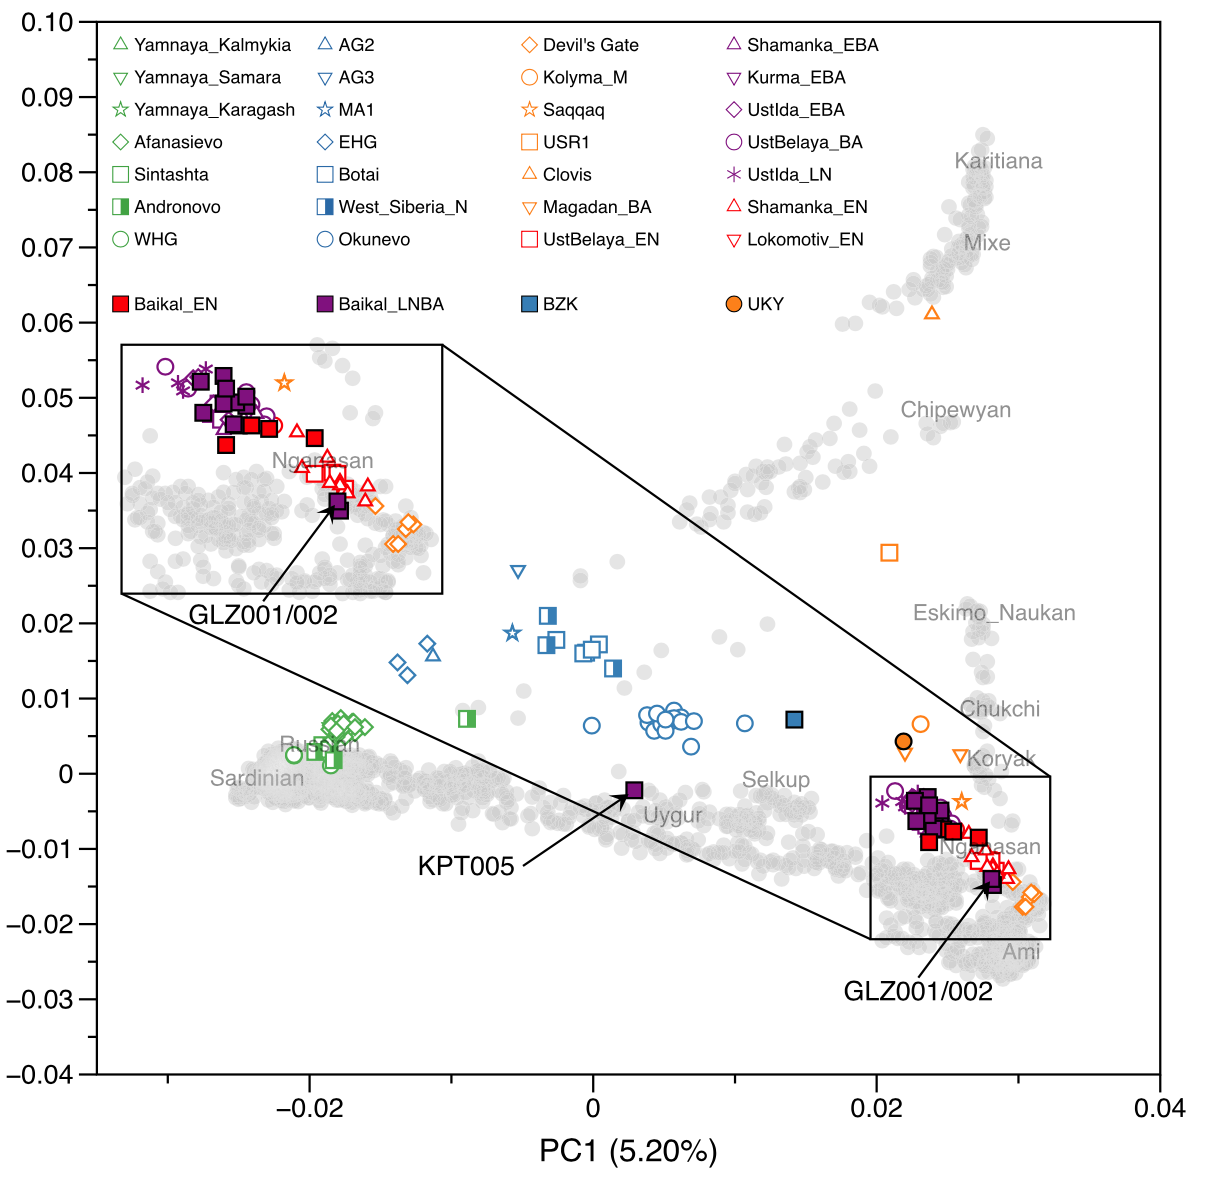
\includegraphics[width=1.1\linewidth]{yu20-pca.png}
    \column{0.4\textwidth}
    \raggedleft
    Ancient Siberians similar to modern ones.

    \bigskip

    Along the line from ``Northeast Asian''
    (\textcolor{orange}{lower right}) and ``Ancient
    North Eurasians'' (\textcolor{cyan}{upper left}).


    \bigskip

    New Paleolithic genome:~\textcolor{orange}{$\bullet$}

  \end{columns}
\end{frame}

\begin{frame}
  \frametitle{Principal Components Inset}
  \begin{columns}
    \column{0.6\textwidth}
    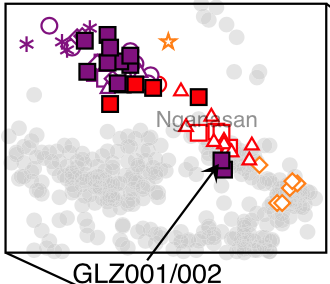
\includegraphics[width=1.1\linewidth]{yu20-pca-inset.png}
    \column{0.4\textwidth}
    \raggedleft
    \textcolor{red}{Early Neolithic} closer to
    \textcolor{orange}{Northeast Asian}.

    \bigskip

    \textcolor{violet}{Late Neolithic/Bronze Age} closer to
    \textcolor{cyan}{Ancient North Eurasian} (off map to NW).

    \bigskip

    Suggests gene flow from ANE into Baikal region after Neolithic.
  \end{columns}
\end{frame}

\begin{frame}
  \frametitle{Admixture Analysis}
  \begin{columns}
    \column{0.5\textwidth}
    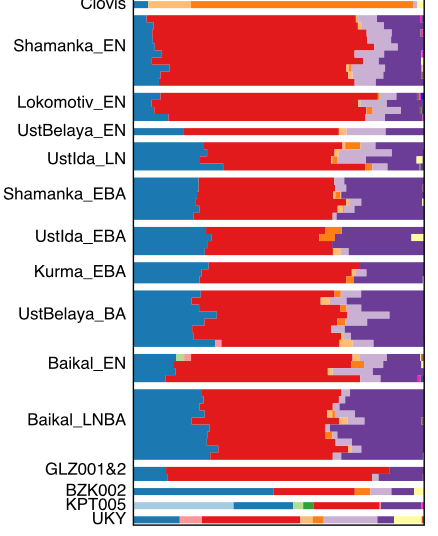
\includegraphics[width=1.1\linewidth]{yu20-struct.png}
    \column{0.5\textwidth}
    \raggedleft
    Mixture \textcolor{NavyBlue}{Ancient North Eurasian},
    \textcolor{red}{Northeast Asian}, and
    \textcolor{violet}{Nganasan}.

    \bigskip

    ANE $\nearrow$; NEA $\searrow$.

    \bigskip

    KPT005 is an immigrant.

    \bigskip

    \textbf{Immigrants}: GLZ001 \& 2 are early Bronze Age but have a
    lot of \textcolor{red}{NEA}. GLZ001 has non-local strontium
    isotope ratios.

    \bigskip

   Implies long-range mobility during this period.
  \end{columns}
\end{frame}

\begin{frame}
\frametitle{Affinities of Mal'ta (24~kya) with world populations}
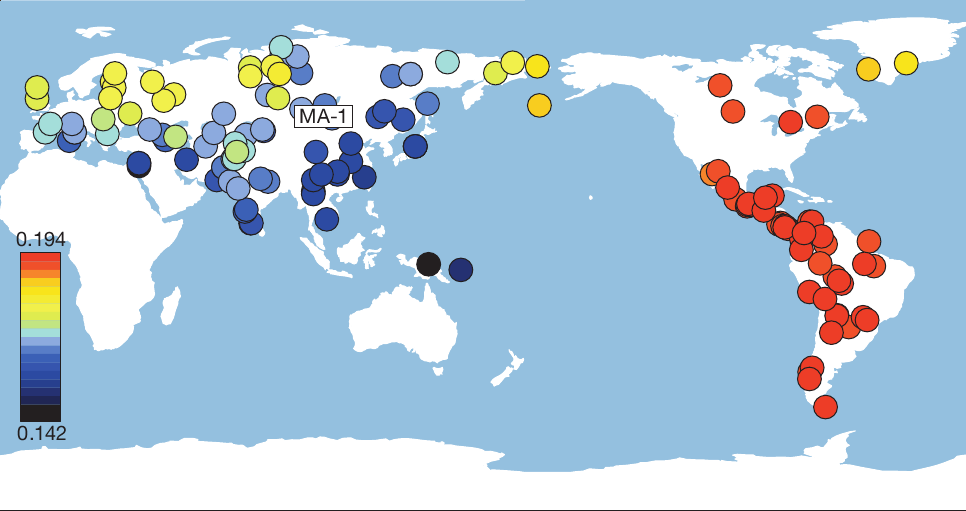
\includegraphics[width=\linewidth]{malta-affinity.png}\\
\mbox{} \hfill {\small (Raghavan et al.{} 2013)}\\[1ex]
Similar to Amerindians and Northern European. ``Ancient North
Eurasians'' (ANE).
\end{frame}

\begin{frame}
\frametitle{Affinities of UKY (14~kya) with world populations}
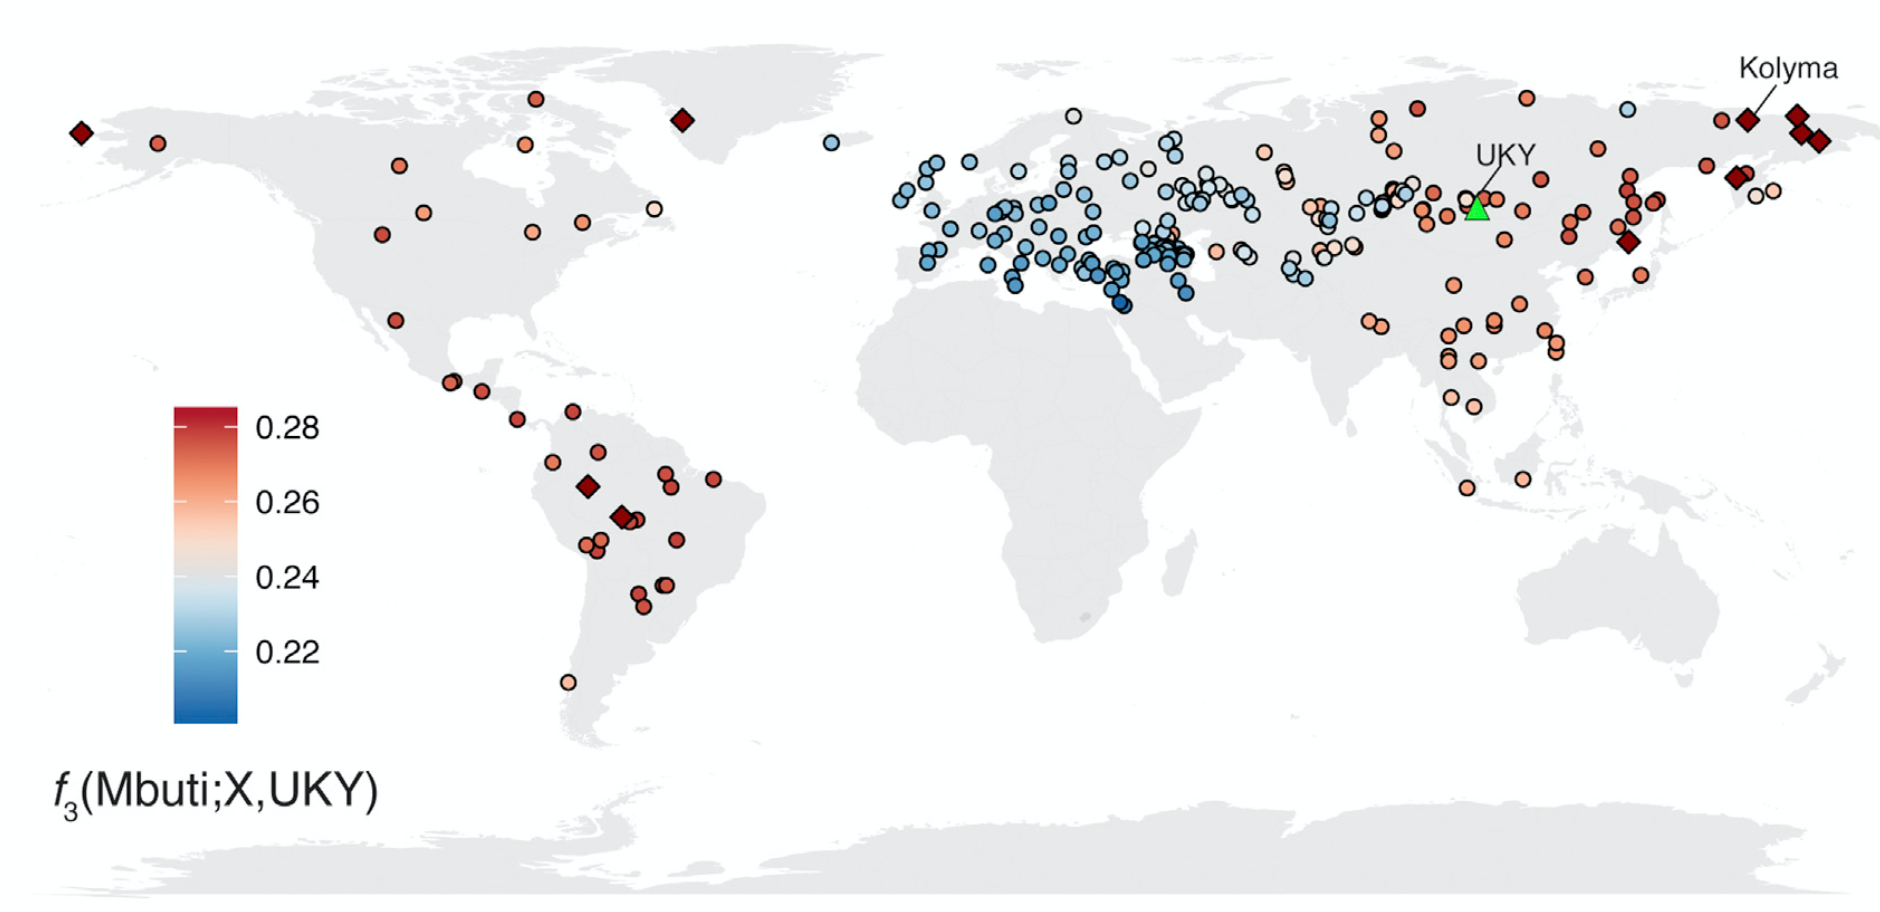
\includegraphics[width=\linewidth]{yu20-UKYaffinity.png}\\
\mbox{} \hfill {\small (Yu et al.{} 2020)}\\[1ex]
Similar to Amerindians and E Asians, not to Europeans.
\end{frame}

\begin{frame}
  \frametitle{Plague DNA}

  Found \emph{Yersina pestis} DNA in two Early Bronze Age individuals
  (GLZ001 \& GLZ002, $\sim$4,400~BP).

  \bigskip

  DNA suggests this strain of plague was not good at transmission via
  fleas.
\end{frame}

\begin{frame}
  \frametitle{Gradual gene flow over millenia}

  Other studies have used genetic data to document fairly sudden
  and nearly complete replacement of one population by another.

  \bigskip

  This article tells a different story: the Ancient Northeast Asian
  DNA of Malt'a~1 (24~kya) survived in this region throughout the
  Upper Paleolithic, as revealed in the UKY specimen (14~kya), and
  even into the Early Neolithic.

  \bigskip

  Furthermore, evolutionary changes between the Early Neolithic and
  Bronze Age were also gradual, suggesting prolonged weak gene flow.

  \bigskip

  Under what circumstances are such changes gradual rather than
  sudden? We have no theory of this.
\end{frame}

\begin{frame}
  \frametitle{Problem~1: Ascertainment bias}

  I worry that these estimates may be affected by the bias that ensues
  when some loci are selected for capture and others are excluded.

\end{frame}  

\begin{frame}
  \frametitle{Problem~2: Goodness of fit}

  In other fields, people routinely ask how well their models fit the
  data.

  \bigskip

  They also use residuals to diagnose problems with fit.

  \bigskip

  Anthropological geneticists seldom do this in studies of population
  history.
\end{frame}

\begin{frame}
  \frametitle{Problem~3: Overfitting}
  \begin{columns}
    \column{0.5\textwidth}
    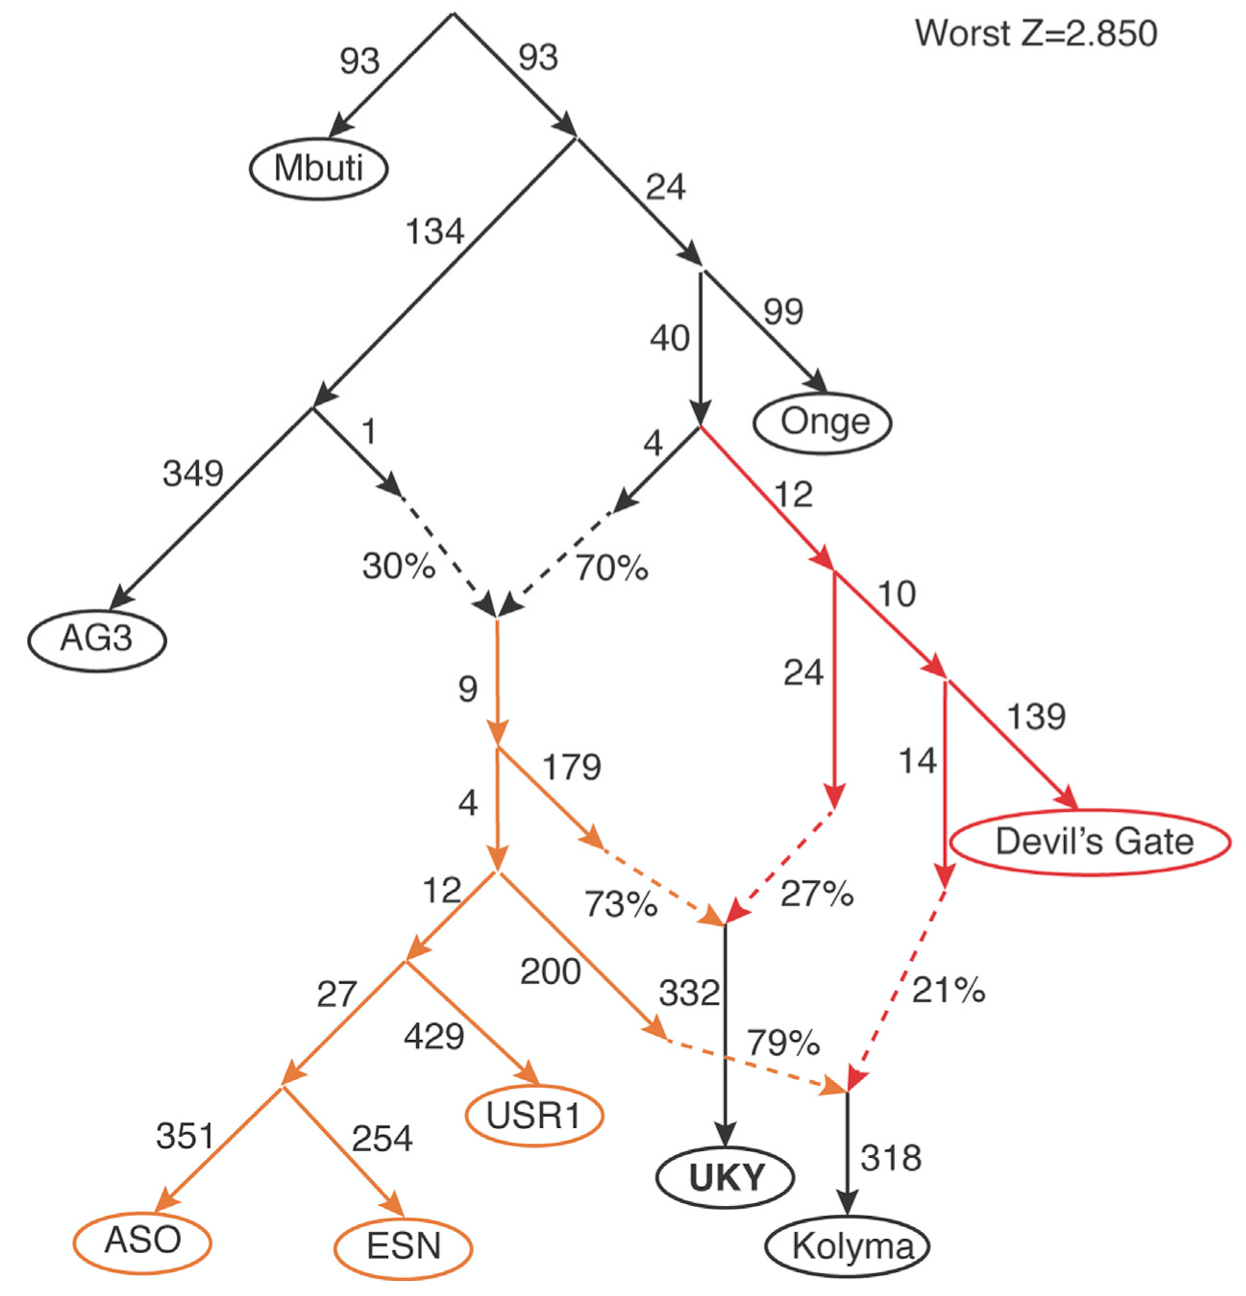
\includegraphics[width=\linewidth]{yu20-network.png}
    \column{0.5\textwidth}
    \raggedleft
    Overfitting happens when you fit noise rather than signal and end
    up with the wrong model.

    \bigskip

    A real danger with complex models.

    \bigskip

    Statisticians have methods that protect against
    overfitting, and geneticists ought use them.
\end{columns}    
\end{frame}

\begin{frame}
  \frametitle{Discussion questions}
  \begin{enumerate}
    \item If the capture array overrepresents SNPs with high
      heterozygosity, what effect might that have on this analysis?
    \item In some regions, population replacements were relatively
      fast and relatively complete. In others (including Baikal), they
      were slow and gradual. Under what circumstances should we expect
      one rather than the other?
  \end{enumerate}
\end{frame}

\end{document}


